%%%%%%%%%%%%%%%%%%%%%%%%%%%%%%%%%%%%%%%%%%%%%%%%%%%%%%%%%%%%%%%%%%%
% Result
% Team:
% Union
% Members: 
% Bernie Huang, Jim Lan, Hoang Tan, Kenny Hsu, Rahul Aditya, Tan Phat, Wei
% Relative files:
% Result_Union.tex
% Note:    
% Do not compile this file compile Main.tex to get the pdf file instead.
%%%%%%%%%%%%%%%%%%%%%%%%%%%%%%%%%%%%%%%%%%%%%%%%%%%%%%%%%%%%%%%%%%%

\section{Final Outcome}
\textit{\footnotesize Author:Bernie Huan, Jim Lan, Hoang Tan, Kenny Hsu, Rahul Aditya, Tan Phat, Wei.}\\
	\begin{enumerate}
		\item Readable PDF on convenient software.
		\item User friendly format for searching.
		\item Free database contains 10k full text.
		\item The most important sentences can be viewed.
		\item It’s more convenient for readers by categorizing articles by fields.
	\end{enumerate}
	
\section{Work Break Structure(WBS)}
	\subsection*{Level 1}
	Website for search, read online and download.
	\subsection*{Level 2}
		\begin{enumerate}
			\item Database for 10k articles(PDF).
			\item Xml file with necessary  information.
			\item PDF which could show in Utopia.
			\item PDF which could show in Utopia.
		\end{enumerate}	
	\subsection*{Level 3}	
		\subsubsection*{Database}
			\begin{enumerate}
				\item Web crawler.
				\item Sever.
				\item Management system.
			\end{enumerate}	
		\subsubsection*{Xml information}
			\begin{enumerate}
				\item Journal name.
				\item Title.
				\item Authors. 
				\item Abstraction.
				\item References URL.
				\item Issue of publication.
				\item Page number.
				\item Place of publication.
				\item ISBN.
				\item Doi.
				\item Date of publication.
			\end{enumerate}	
		\subsubsection*{Xml information}
			\begin{enumerate}
				\item List of data.
				\item Search engine.
				\item API. 
				\item User account.
			\end{enumerate}	

%\begin{center}
%	\includegraphics[width=\columnwidth]{Union_Background_Chart_2
%\end{center}

%\begin{center}
  %\includegraphics[width=\columnwidth]{Table for method Union}.\\
  %\includegraphics[width=\columnwidth]{Table 2 for method Union}.\\
  %\caption{Result of finding all forms of "abstract", "introduction" written by different authors}
%\end{center}

\section*{Describe process}
	\subsection*{Journal name, Title, Authors, Abstract, Reference URL extraction}
		\begin{enumerate}
			\item Import some necessary packages.
			\item Convert PDF file into TXT file.
			\item Detect the Journal name, Title, Authors, Abstraction, Reference URL -database's words.
			\item Capture the Journal name, Title, Authors, Abstraction, Reference URL  in the TXT files by python.
			\item Output the Journal name, Title, Authors, Abstraction, Reference URL  of the article in TXT file.
		\end{enumerate}	

\begin{figure}[tbh]
	\begin{center}
		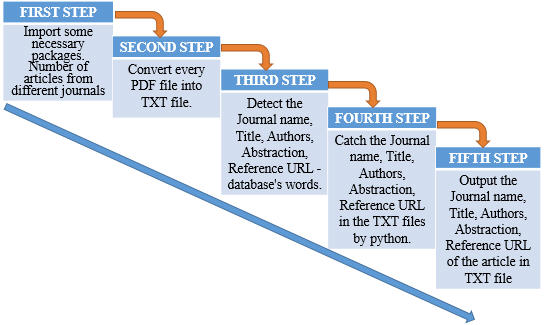
\includegraphics[width=\columnwidth]{Union_Method_Chart_Extraction}
	\end{center}
	\caption{The Extracton.}
\end{figure}

	\subsection*{Search engine and API}
	The search sentence part or word is related to the search engine. 
	After extracting the necessary information, we have to find a way to search these data.
		\begin{enumerate}
			\item Convert PDF file into TXT file.
			\item Read the txt files by lines.
			\item The array is created to divide the section of the articles.
			\item The array is expanded to divide the section clearly.
			\item Users search the sentences, the program search all sections by this sentence.
			\item Output the result.
		\end{enumerate}	

\begin{figure}[tbh]
	\begin{center}
		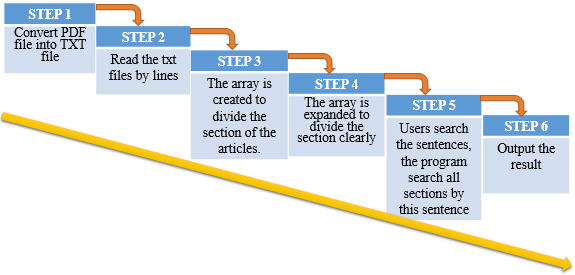
\includegraphics[width=\columnwidth]{Union_Method_Chart_Search engine}
	\end{center}
	\caption{The search engine.}
	\end{figure}
	
\section*{Result and Discussion}
	\subsection*{Journal name, Title, Authors, Abstract, Reference URL extraction}
	The result of these part, we tranfer to TXT file, you can see in figure.

	\begin{figure}[tbh]
		\begin{center}
			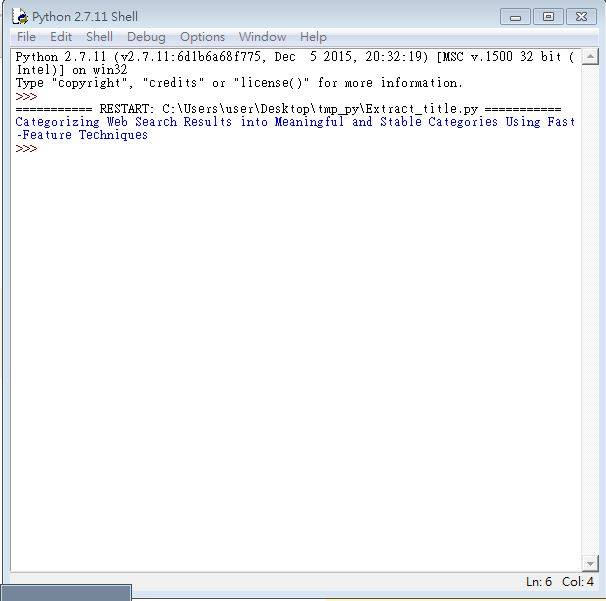
\includegraphics[width=\columnwidth]{Union_Result_Chart_Title}
		\end{center}
		\caption{The result of title.}
	\end{figure}
	
	\begin{figure}[tbh]
		\begin{center}
			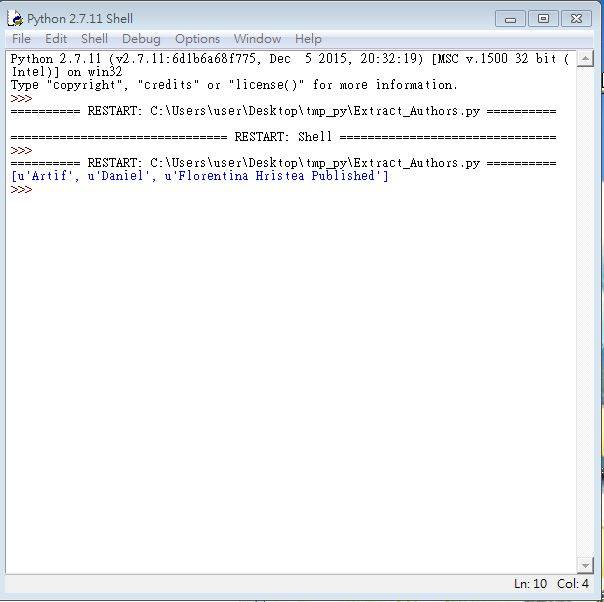
\includegraphics[width=\columnwidth]{Union_Result_Chart_Author}
		\end{center}
		\caption{The result of author.}
	\end{figure}
	
	\begin{figure}[tbh]
		\begin{center}
			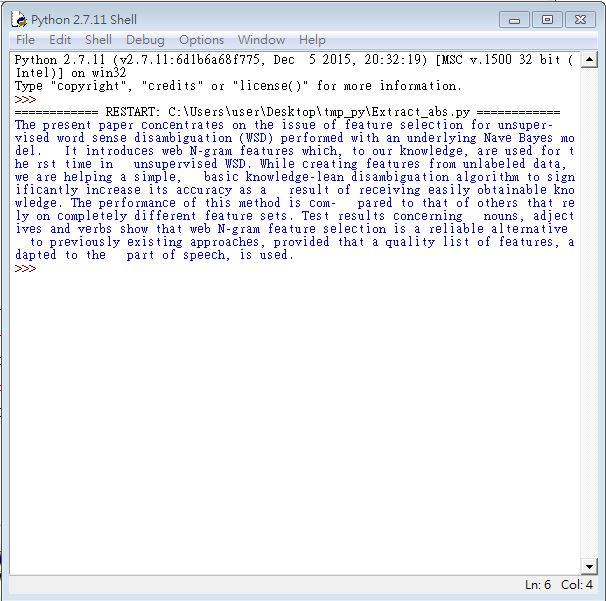
\includegraphics[width=\columnwidth]{Union_Result_Chart_Abstract}
		\end{center}
		\caption{The result of abstract.}
	\end{figure}
	
	\subsection*{Search engine and API}
	Search engine have run, but we only apply with one PDF file and you can see the result in figure. 

	\begin{figure}[tbh]
		\begin{center}
			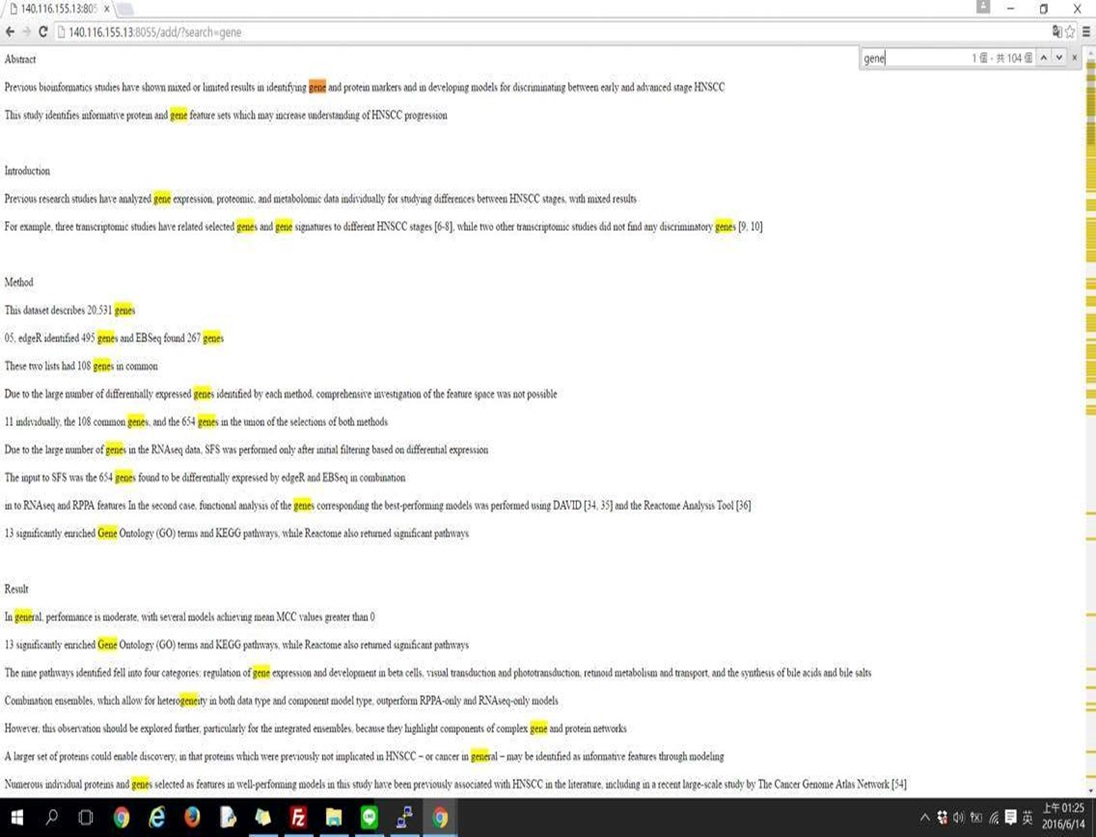
\includegraphics[width=\columnwidth]{Union_Result_Chart_Search engine}
		\end{center}
		\caption{The result of search engine.}
	\end{figure}

	\begin{figure}[tbh]
		\begin{center}
			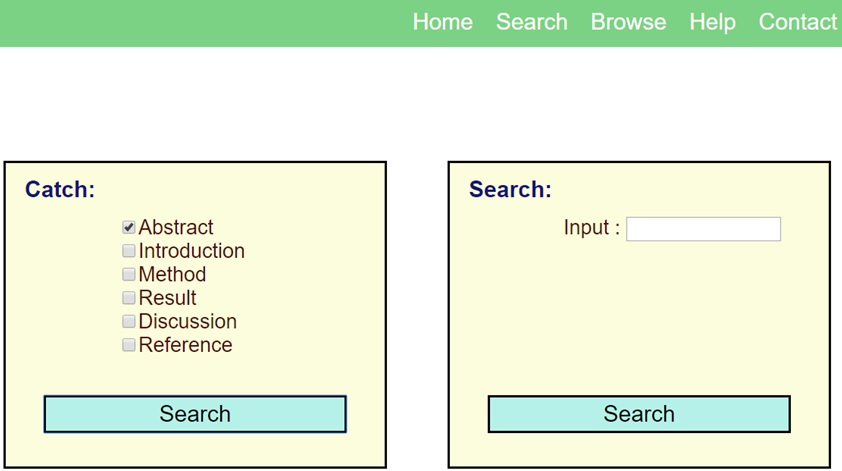
\includegraphics[width=\columnwidth]{Union_Result_Chart_API}
		\end{center}
		\caption{The result of API.}
	\end{figure}

	We also attempt to produce an semi-automatic interface that help users to inquire certain information from our database. 
	Currently it allows user to search for abstracts, introduction, method, result, discussion, and reference. 
	We will continue develop the interface in the remaining week. 
	The objectives are either covering more functions or make the results pages has more professional appearance. 
	However, that being said when we still have enough time.
	
\section*{Working Plan}

\begin{figure}[tbh]
	\begin{center}
		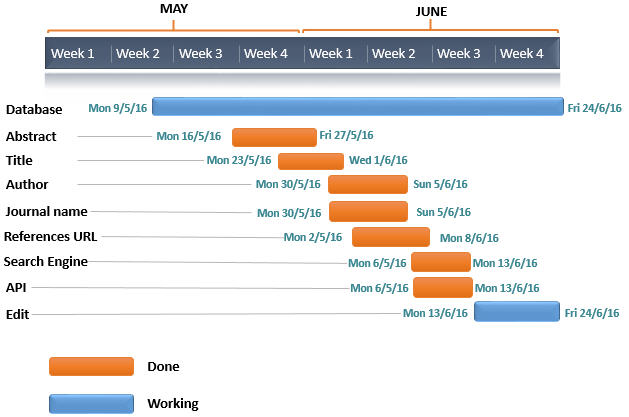
\includegraphics[width=\columnwidth]{Union_Result_Chart_working plan}
	\end{center}
	\caption{The working plan.}
	\end{figure}
	
\section*{Conclusion}
As mentioned in the background, our team used natural language processing in order to generate metadata. 
The scope of metadata processing is about producing at least three types of metadata including author name, title and abstract. 
This is the least we want to do within the time frame of this course. 

		\begin{enumerate}
			\item The result of author name extraction, we use the existing python packages to achieve our goal.
			The key point in this part is natural language processing, which we have introduced in the basic section. 
			Also we combine the key word comparison technique to finish this task.
			\item The result of title extraction, We chose python to be the program to catch the title, we also shown method and result in some figure above.
			\item The result of title extraction, developing from previous theory mentioned in the background section, 
			we use the python to catch the abstract.
		\end{enumerate}	
Once accomplishing the 3 types of metadata, we will extend the scope of our project, intimidate the scheme to produce other remaining metadata such as doix number, journal name, volume number and so on. 
		\begin{enumerate}
			\item (Search engine) About the search sentence part is related to the search engine. After extracting the necessary information, we had to find out a way to search these data. The result is also shown above.
			\item (API) We also attempt to produce a semi-automatic interface that help users to inquire certain information from our database.
		\end{enumerate}	

\section*{Suggestion}
If time is still on our side, we will even extend the scope of our project further and join other teams to produce a search engine. 
Following discussion are our plan to complete extracting the 4 first types of metadata from PDF files.
We will continue developing this interface if we have enough time. 
The objectives are either covering more functions or make the results pages has more professional appearance.
 
\newpage % Ends the current page and causes all figures and tables to be printed